\chapter{Работа и мощность сил приложенных к твердому телу при поступательном,
вращательном, сферическом и свободном движении твердого тела. Работа
внутренних сил твердого тела.}

\section{Работа и мощность сил приложенных к твердому телу при поступательном, 
вращательном и сферическом движении твёрдого тела}

\emph{Элементарная работа сил, приложенная к материальной точке, равна сумме 
элементарных работ этих сил.}
\[ 
	dA = \left( \vec{F_1} + \vec{F_2} + ... + \vec{F_n} \right)\cdot d\vec{r} =
	dA(\vec{F_1}) + dA(\vec{F_2}) + ... + dA(\vec{F_n})
\]

\begin{figure}[h!]
    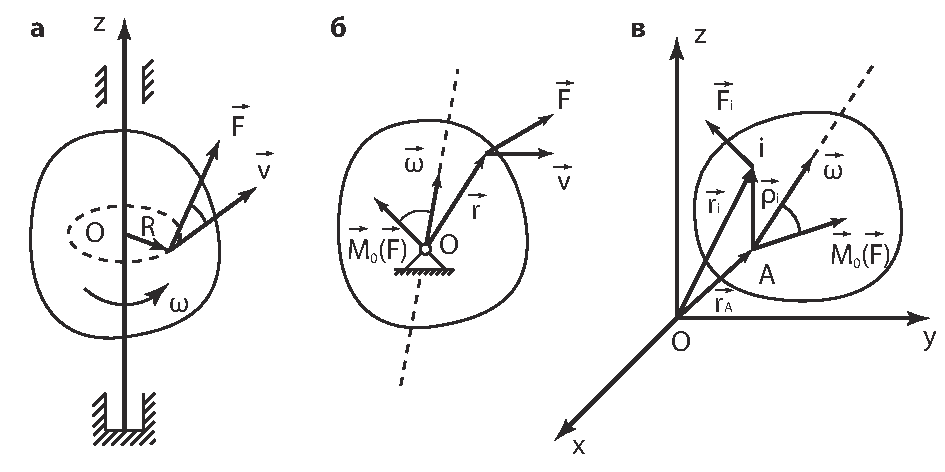
\includegraphics[width=.47\textwidth]{53_01}
    \parbox{.47\textwidth}{\caption{} \label{pic53_01}}
\end{figure}

При поступательном движении твёрдого тела его можно принять за материальную 
точку и для вычисления работы силы, приложенной к нему, применять все 
формулы для подсчёта элементарной и полной работы силы, приложенной к 
материальной точке.

При вращении твёрдого тела вокруг неподвижной оси скорость точки, где приложена 
сила \( F \) (рис. \ref{pic53_01}а), равна \( v = \omega R \). По формуле
\[ 
	dA(\vec{F}) = \vec{F}\cdot\vec{v}dt = Fv\cos\Hat{\vec{F}\vec{v}} = 
	F\omega R\cos{\Hat{Fv}}
\]
Вектор скорости лежит в плоскости, перпендикулярной оси вращения и оси \( Oz \), 
поэтому \( |F\cos\Hat{Fv}| = F_p \), где \( F_p \) -- модуль проекции силы на эту 
плоскость. 

Следовательно, по определению момента силы относительно оси 
\( |M_z(F)| = F_p R\), то есть \( FR\cos\Hat{Fv} = \pm M_z(F) \).

Поэтому элементарную работу силы, приложенной к телу, вращающемуся вокруг 
неподвижной оси, можно выразить так:
\[ dA(\vec{F}) = \pm M_z(\vec{F})\omega dt = \pm M_z(\vec{F})d\phi \]
где \( d\phi = \omega dt \) -- элементарный угол поворота тела.

Мощность в случае вращения твёрдого тела вокруг неподвижной оси 
вычисляется так:
\[ N(\vec{F}) = \frac{dA(\vec{F}}{dt} = \pm M_z(\vec{f})\omega \]

При вращении твёрдого тела вокруг неподвижной точки 
(сферическое движение) (рис. \ref{pic53_01}б) скорость \( v \) точки 
приложения силы \( F \) можно выразить по 
формуле Эйлера, согласно которой \( v = \omega\times r \), где 
\( r \) -- радиус-вектор точки приложения, а \( \omega \) -- 
мгновенная угловая скорость тела. Тогда:
\[ 
	dA(\vec{F}) = \vec{F}\cdot\vec{v}dt = 
	\vec{F}\cdot\left( \vec{\omega}\times\vec{r} \right)dt =
	\vec{\omega}\cdot\left( \vec{r}\times\vec{F} \right)dt
\]
так как по свойству смешанного произведения векторов 
\( F\cdot\left( \omega\times r) = \omega\cdot\left( r\times F\right) \). 
Но \( r\times F = M_0(F) \) -- момент силы относительно точки или 
центра \( O \). Поэтому 
\[ 
	dA(\vec{f}) = \vec{\omega}\cdot M_0(\vec{F})dt = 
	M_0(\vec{F}\cdot\omega\cos\Hat{M_0\left( \vec{F} \right)}dt =
	M_\omega(\vec{F})\omega dt = M_\omega(\vec{F})d\phi
\]
где \( d\phi \) -- элементарный угол поворота вокруг мгновенной оси 
вращения, а \( M_\omega(F) = M_0(F)\cos\Hat{M_0(F)\omega} \) -- 
проекция вектора \( M_0(F) \) на направление мгновенной угловой 
скорости, которую называют \emph{моментом силы относительно мгновенной 
оси вращения}.

Мощность силы в этом случае можно выразить так:
\[ 
	N(\vec{F}) = \frac{dA(\vec{F}}{dt} = 
	\vec{M_0(\vec{F}}\cdot\vec{\omega} =
	M_\omega(\vec{F})\cdot\omega
\]

\section{Работа внутренних сил твердого тела + свободное движение}

В самом общем случае (рис. \ref{pic53_01}в), когда на свободное твёрдое тело 
действует система сил \( \left( F_1, F_2, ..., F_n \right) \) скорость 
точки \( v_i \) точки тела с номером \( i \), на которую действет сила 
\( F_i \), можно выразить как 
\( \vec{v_i} = \vec{v_A} + \vec{\omega}\times\vec{\rho_i} \), 
где \( v_A \) -- скорость полюса \( A \), \( \rho_i \) -- радиус-вектор 
точки относительно полюса. Тогда для элементарной работы системы сил 
получим выражение:
\[ 
	dA = \sum_{i=1}^{N} \vec{F_i}
	\left( \vec{v_a} + \vec{\omega}\times\vec{\rho_i} =
	\left( \sum_{i=1}^{N}\vec{F_i} \right)\cdot\vec{v_A}dt + 
	\sum_{i=1}^{N}\vec{F_i}\cdot\left( \vec{\omega}\times\vec{\rho_i} \right)dt
\]

Воспользовавшись свойствами смешанного произведения векторов, перепишем 
выражение в виде:
\[ 
	dA = \left( \sum_{i=1}^{N}\vec{F_i} \right)\cdot\vec{v_A}dt + 
	\left( \sim_{i=1}^{N} \vec{\rho_i}\times\vec{F_i}\right)\cdot\vec{\omega}dt = 
	\left( \sum_{i=1}^{N}\vec{F_i} \right)\cdot\vec{v_A}dt + 
	\left( \sum_{i=1}^{N} \vec{M_A(\vec{F_i})} \right)\cdot\vec{\omega}dt
\]

Считая твёрдое тело неизменяемой системой материальных точек, разделим силы, 
действующие на его точки, на внешние и внутренние, то есть 
\( F_i = F^e_i + F^i_i \). Подставляя в предыдущее равенство получаем:
\[ 
	dA = \left( \sum_{i=1}^{N} \vec{F^e_i} \right)\cdot\vec{v_A}dt + 
	\left( \sum_{i=1}^{N} \vec{M_A(\vec{F^e_i})} \right)\cdot\vec{\omega}dt +
	\left( \sum_{i=1}^{N} \vec{F^i_i} \right)\cdot\vec{v_A}dt + 
	\left( \sum_{i=1}^{N} \vec{M_A(\vec{F^i_i})} \right)\cdot\vec{\omega}dt
\]

В последнем выражении главный вектор и главный момент внутренних сил 
твёрдого тела, согласно свойствам внутренних сил системы, равны нулю:
\[ 
	\sum\vec{F^i_i} = \vec{R^i} = 0;\quad 
	\sum\vec{M_A(\vec{F^i_i})} = \vec{M^i_A} = 0
\]

Следовательно, \emph{элементарная \( dA^i\) и полная работа \( A^i \), 
а также мощность \( N^i \) внутренних сил абсолютно твёрдого тела 
равна нулю.}

\newpage
